\documentclass{classrep}
\usepackage[utf8]{inputenc}
\frenchspacing

\usepackage{graphicx}
\usepackage[usenames,dvipsnames]{color}
\usepackage[hidelinks]{hyperref}
\usepackage{lmodern}
\usepackage{placeins}
\usepackage{url}
\usepackage{amsmath, amssymb, mathtools}
\usepackage{listings}
\usepackage{fancyhdr, lastpage}

\pagestyle{fancyplain}
\fancyhf{}
\renewcommand{\headrulewidth}{0pt}
\cfoot{\thepage\ / \pageref*{LastPage}}

%--------------------------------------------------------------------------------------%
\studycycle{Informatyka stosowana, studia dzienne, II st.}
\coursesemester{II}

\coursename{Analiza danych złożonych}
\courseyear{2021/2022}

\courseteacher{dr hab inż. Agnieszka Duraj}
\coursegroup{środa, 11:00}

\author{%
    \studentinfo[239671@edu.p.lodz.pl]{Jan Karwowski}{239671}\\
    \studentinfo[239676@edu.p.lodz.pl]{Kamil Kowalewski}{239676}\\
}

\title{Zadanie 2.: Grupowanie danych}

\begin{document}
    \maketitle
    \thispagestyle{fancyplain}

    \tableofcontents
    \newpage

    \section{Cel} {
        Celem zadania jest dokonania grupowania i odnalezienia wzorców wyjątkowych
        poprzez wykorzystanie metody grupowania opartej na odległości oraz metody
        grupowania hierarchicznego.
    }

    \section{Zbiory danych} {
        Do przeprowadzenia badań w tym zadaniu zostały wykorzystane trzy zbiory danych,
        dwa z nich są zbiorami naturalnymi natomiast jeden z nich jest sztucznie
        wygenerowany.

        Zbiór wygenerowany sztucznie został utworzony poprzez wybranie dwóch punktów na
        płaszczyźnie dwuwymiarowej i wylosowanie dla każdego z nich 200 punktów we
        względnie bliskim otoczeniu. Następnie do tak utworzonego zbioru danych
        dołączonych zostało 20 punktów, których pozycje losowane były ze zdecydowanie
        większego zakresu niż poprzednich 400 punktów - są to sztucznie wygenerowane
        wyjątki.

        Drugi i trzeci zbiór danych pochodzą z serwisu \emph{Outlier Detection
        DataSets} \cite{odds}, który zawiera kilkadziesiąt przykładowych zbiorów
        danych, dostosowanych do zadania wyszukiwania wyjątków. Zbiory te są już
        znormalizowane i oczyszczone, każdy przykład w każdym zbiorze jest oznaczony
        jedną z dwóch klas: wyjątek lub nie wyjątek. Wybranymi zbiorami są ,,http''
        oraz ,,mammography''.

        Zbiór ,,http'' zawiera 3 kolumny i oryginalnie ponad 500 tys. wierszy, z czego
        ok. 0.4\% stanowią wyjątki. Zbiór ten na potrzebny niniejszego zadania został
        ograniczony do ok 1\% próbek, przy czym proporcja wyjątków została zachowana.
        Zbiór ten zawiera informacje o zapytaniach HTTP.

        Zbiór ,,mammography'' zawiera 6 kolumn i ponad 11 tys. wierszy, z czego ok. 2\%
        stanowią wyjątki. Zbiór ten dotyczy wyników badania mammograficznego i
        wyjątkami są przypadki zdiagnozowane jako chore, których jest stosunkowo mało
        do przypadków zdrowych, przez co zbiór ten został dostosowany do zadania
        rozpoznawania wyjątków, chociaż oryginalnie dotyczy zadania klasyfikacji.
    }

    \section{Implementacja} {
        Program został napisany w języku Python z wykorzystaniem biblioteki
        scikit-learn\cite{sklearn} aby skorzystać z gotowych implementacji algorytmów.
        Wybranymi algorytmami są:
    % @formatter:off
        \begin{itemize}
            \item K-średnich (ang. KMeans)
            \item Metoda aglomeracyjna (ang. Agglomerative Clustering)
            \item DBSCAN (ang. Density Based Spatial Clustering of Applications with Noise)
            \item LOF (ang. Local Outlier Factor)
        \end{itemize}
    % @formatter:on
        Do kodu źródłowego jest dołączony skrypt \textit{run.sh} zawierający wszystkie
        kombinacja parametrów użyte do badań natomiast wyniki w postaci wykresów są
        zapisywane do plików.
    }

    \section{Opis algorytmów} {

        \subsection{K-średnich} {
            Algorytm K-średnich należy do metody grupowania opartego na odległości.
            Jego działania rozpoczyna się od podziału zbioru przypadku na \textit{K}
            skupień i rozpoczyna działanie od losowo wybranych \textit{K} środków
            skupień, które są możliwie jak najbardziej od siebie oddalone. W czasie
            kolejnych iteracji przypisuje obiekty do najbliższych skupień. Sama
            odległość jest wyliczana na podstawie wybranej metryki np. euklidesowej. Po
            dokonaniu alokacji obiektu są wyznaczane nowe środku skupień i na tej
            podstawie jest przypisywany kolejny obiekt. Kroki te są powtarzane do
            uzyskania stabilizacji lub gdy funkcje kryterialne nie osiągną swojego
            minimum.
        }

        \subsection{Metoda aglomeracyjna} {
            Metoda aglomeracyjna należy do grupy algorytmów hierarchicznych.
            Zakłada on na początku, że każda próbka jest osobnym klastrem. W
            kolejnych iteracjach łączy najbliższe siebie klastry w jeden. W ten sposób
            z każdą iteracją jest jeden klaster mniej. Algorytm kończy się, kiedy
            powstanie zadana liczba klastrów, w skrajnym przypadku jeden. Podobieństwo
            klastrów mierzy się z wykorzystaniem odpowiedniej metryki (np. euklidesowej
            bądź miejskiej) i odpowiedniej metody łączenia. Te dwa parametry mają
            zasadniczy wpływ na działanie algorytmu. Trzecim badanym parametrem jest
            liczba klastrów, na której algorytm się zatrzymuje. Oczywiście aby osiągnąć
            zadaną liczbę klastrów K dla N próbek, algorytm aglomeracyjny musi przejść
            przez wszystkie całkowite liczby klastrów od N do K.
        }

        \subsection{DBSCAN} {
            Algorytm DBSCAN należy do grupy algorytmów gęstościowych, które przyjmują
            gęstość jako lokalne kryterium grupowania. Celem samego algorytmu jest
            identyfikacja regionów z dużą liczbą punktów. Posiada on dwa parametry
            \textit{epsilon} czyli promień sąsiedztwa punktu \textit{x} oraz
            \textit{minimum points} czyli minimalną liczbę punktów, które muszą być we
            wcześniej wspomnianym promieniu. Można wyróżnić 3 rodzaje punktów,
            pierwszym z nich są te, które są w promieniu i parametr
            \textit{minimum points} jest spełniony. Są wtedy nazywane punktami
            rdzeniowymi. Drugim rodzajem są punkty graniczne czyli te, które leżą w
            promieniu lecz nie \textit{minimum points} nie jest spełniony. Ostatnim
            przypadkiem punktu jest punkt szumu, które nie spełnia obu wcześniej
            wspomnianych warunków. Za pośrednictwem właśnie punktów szumu będą
            odnajdywane wzorce wyjątkowe.
        }

        \subsection{Local Outlier Factor (LOF)} {
            Local Outlier Factor jest algorytmem do wykrywania anomalii czy też wzorców
            wyjątkowych. Jego działanie jest oparte na wyliczaniu odchylenia
            gęstości lokalnej danego punktu w stosunku do jego sąsiadów. Próbki, które
            mają znacznie mniejszą gęstość niż sąsiednie są określane jako jako
            wzorce wyjątkowe. W przypadku biblioteki scikit-learn\cite{sklearn}
            sugerowaną liczbą rozważanych sąsiadów jest wartość \textit{20}.
        }
    }

    \section{Eksperymenty} {

        W ramach realizacji niniejszego zadania przeprowadzonych zostało wiele
        eksperymentów, mających na celu porównania działania omówionych powyżej
        czterech algorytmów do wyszukiwania wyjątków w różnych zbiorach danych.
        Eksperymenty zostały podzielone na trzy serie, każda związana z jednym zbiorem
        danych. W ramach każdej serii zaprezentowane są wyniki pojedynczego
        uruchomienia każdego algorytmu. W rzeczywistości dla każdego algorytmu i dla
        każdego zbioru danych zbadane zostały różne wartości hiperparametrów i wybrany
        został najlepszy ich zestaw. Pośrednie wyniki nie są prezentowane, jako że
        celem tego zadania jest przede wszystkim porównanie algorytmów między sobą.

        \subsection{Http} {
            \begin{figure}[!htbp]
                \centering
                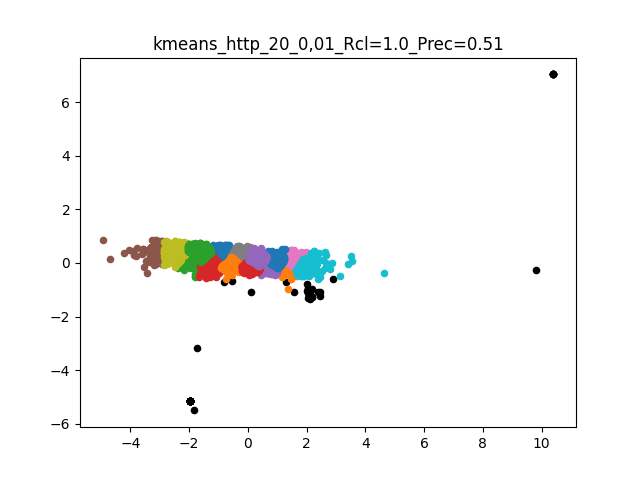
\includegraphics[width=\textwidth]{img/kmeans_http_20_0,01_-115739.png}
                \caption
                {Wyniki klasteryzacji algorytmem kmeans dla zbioru http}
                \label{fig:http_kmeans}
            \end{figure}

            \begin{figure}[!htbp]
                \centering
                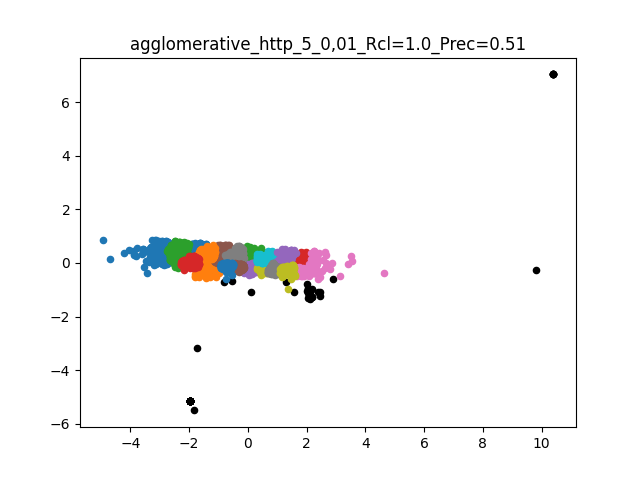
\includegraphics[width=\textwidth]{img/agglomerative_http_5_0,01_-115749.png}
                \caption
                {Wyniki klasteryzacji algorytmem agglomerative dla zbioru http}
                \label{fig:http_agglomerative}
            \end{figure}

            \begin{figure}[!htbp]
                \centering
                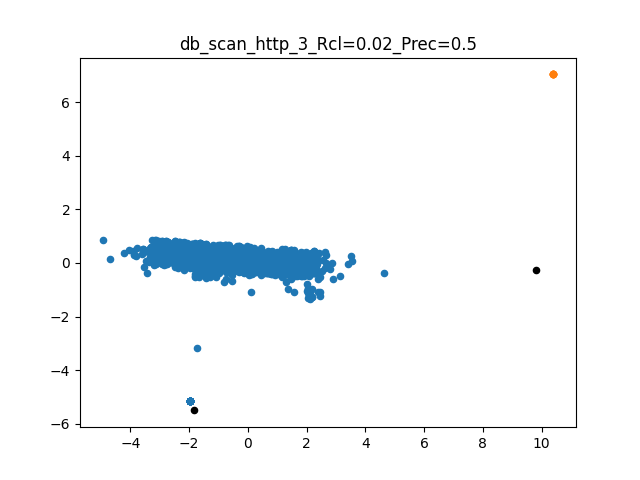
\includegraphics[width=\textwidth]{img/db_scan_http_3_-115804.png}
                \caption
                {Wyniki klasteryzacji algorytmem dbscan dla zbioru http}
                \label{fig:http_dbscan}
            \end{figure}

            \begin{figure}[!htbp]
                \centering
                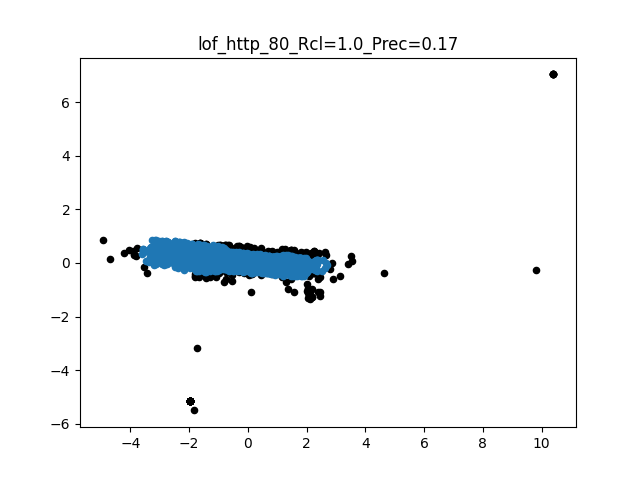
\includegraphics[width=\textwidth]{img/lof_http_80_-115810.png}
                \caption
                {Wyniki klasteryzacji algorytmem lof dla zbioru http}
                \label{fig:http_lof}
            \end{figure}
            \FloatBarrier

            \begin{table}[!htbp]
                \centering
                \begin{tabular}{|c|c|c|c|c|}
                    \hline
                    Algorytm & recall & precision \\ \hline
                    Kmeans &1.0 & 0.51 \\ \hline
                    Agglomerative & 1.0 & 0.51  \\ \hline
                    DBSCAN & 0.02 & 0.5  \\ \hline
                    LOF & 1.0 & 0.17  \\ \hline
                \end{tabular}
                \caption
                {Zestawienie wyników działania algorytmów dla zbioru http}
                \label{tab:http}
            \end{table}
            \FloatBarrier
        }

        \subsection{Mammography} {

            \begin{figure}[!htbp]
                \centering
                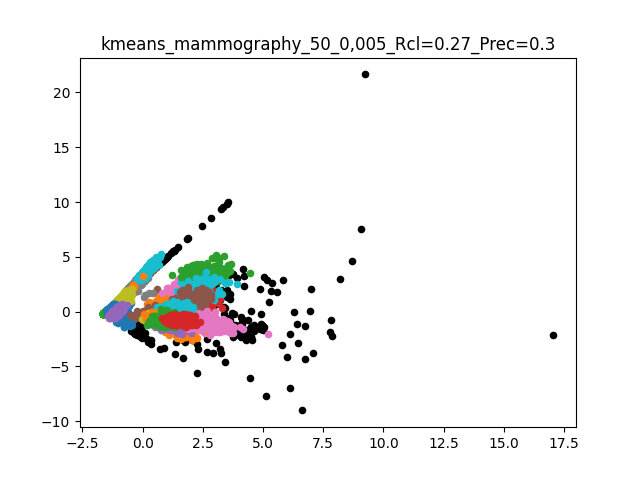
\includegraphics[width=\textwidth]{img/kmeans_mammography_50_0,005_-115816.png}
                \caption
                {Wyniki klasteryzacji algorytmem kmeans dla zbioru Mammography}
                \label{fig:mammo_kmeans}
            \end{figure}

            \begin{figure}[!htbp]
                \centering
                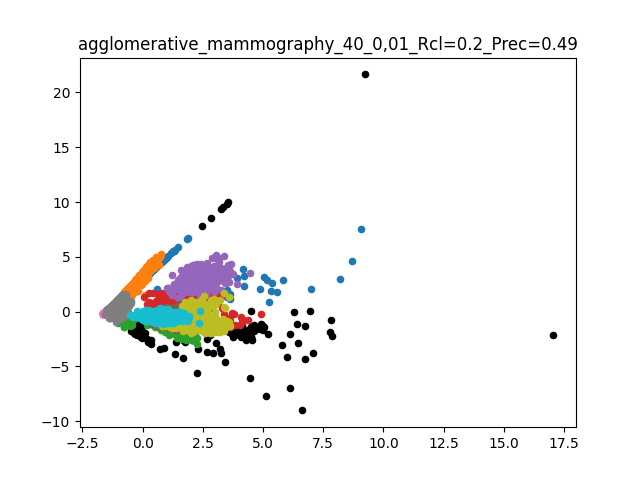
\includegraphics[width=\textwidth]{img/agglomerative_mammography_40_0,01_-115822.png}
                \caption
                {Wyniki klasteryzacji algorytmem agglomerative dla zbioru Mammography}
                \label{fig:mammo_agglomerative}
            \end{figure}

            \begin{figure}[!htbp]
                \centering
                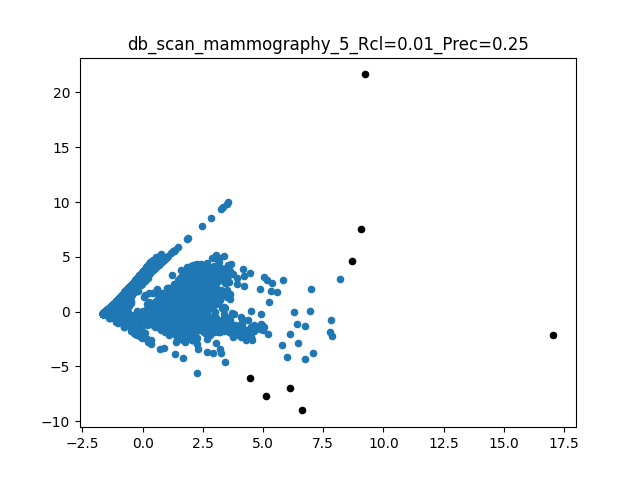
\includegraphics[width=\textwidth]{img/db_scan_mammography_5_-115827.png}
                \caption
                {Wyniki klasteryzacji algorytmem dbscan dla zbioru Mammography}
                \label{fig:mammo_dbscan}
            \end{figure}

            \begin{figure}[!htbp]
                \centering
                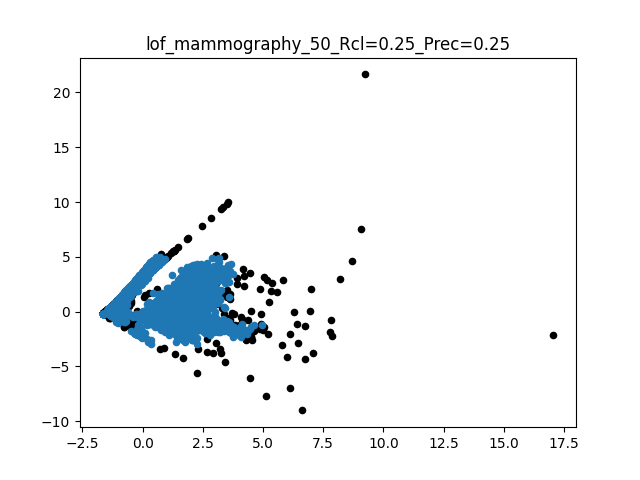
\includegraphics[width=\textwidth]{img/lof_mammography_50_-115830.png}
                \caption
                {Wyniki klasteryzacji algorytmem lof dla zbioru Mammography}
                \label{fig:mammo_lof}
            \end{figure}
            \FloatBarrier

            \begin{table}[!htbp]
                \centering
                \begin{tabular}{|c|c|c|c|c|}
                    \hline
                    Algorytm & recall & precision \\ \hline
                    Kmeans & 0.27 & 0.3  \\ \hline
                    Agglomerative & 0.2 & 0.49  \\ \hline
                    DBSCAN & 0.01 & 0.25  \\ \hline
                    LOF & 0.25 & 0.25  \\ \hline
                \end{tabular}
                \caption
                {Zestawienie wyników działania algorytmów dla zbioru mammography}
                \label{tab:mammo}
            \end{table}
            \FloatBarrier
        }

        \subsection{Synthetic} {

            \begin{figure}[!htbp]
                \centering
                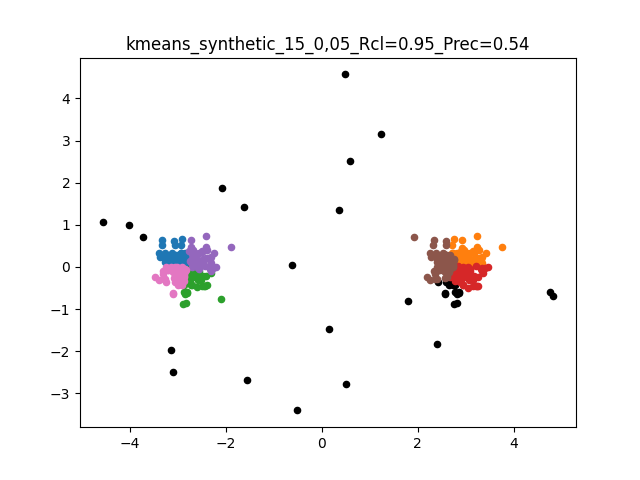
\includegraphics[width=\textwidth]{img/kmeans_synthetic_15_0,05_-115716.png}
                \caption
                {Wyniki klasteryzacji algorytmem kmeans dla zbioru Synthetic}
                \label{fig:synth_kmeans}
            \end{figure}

            \begin{figure}[!htbp]
                \centering
                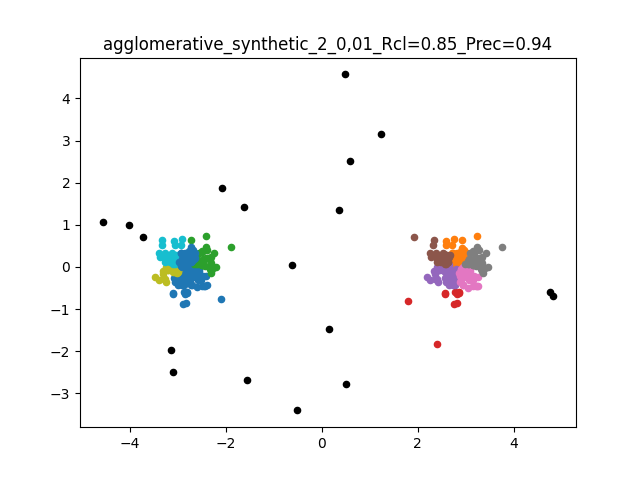
\includegraphics[width=\textwidth]{img/agglomerative_synthetic_2_0,01_-115720.png}
                \caption
                {Wyniki klasteryzacji algorytmem agglomerative dla zbioru Synthetic}
                \label{fig:synth_agglomerative}
            \end{figure}

            \begin{figure}[!htbp]
                \centering
                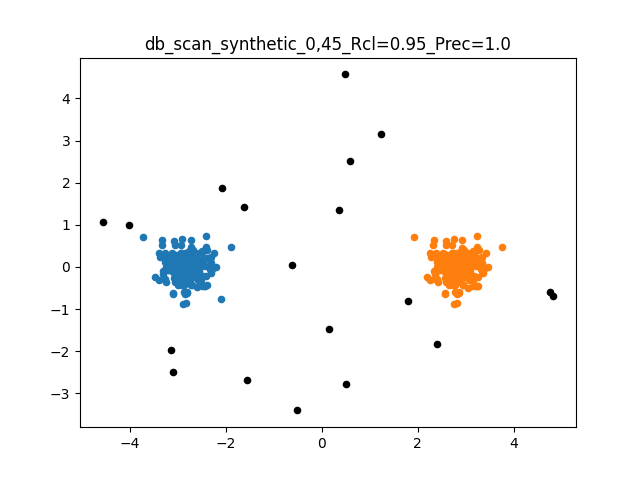
\includegraphics[width=\textwidth]{img/db_scan_synthetic_0,45_-115726.png}
                \caption
                {Wyniki klasteryzacji algorytmem dbscan dla zbioru Synthetic}
                \label{fig:synth_dbscan}
            \end{figure}

            \begin{figure}[!htbp]
                \centering
                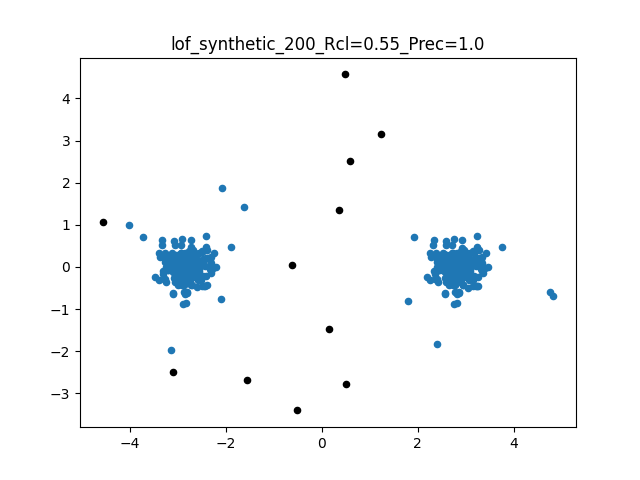
\includegraphics[width=\textwidth]{img/lof_synthetic_200_-115734.png}
                \caption
                {Wyniki klasteryzacji algorytmem lof dla zbioru Synthetic}
                \label{fig:synth_lof}
            \end{figure}
            \FloatBarrier

            \begin{table}[!htbp]
                \centering
                \begin{tabular}{|c|c|c|c|c|}
                    \hline
                    Algorytm & recall & precision \\ \hline
                    Kmeans & 0.95  & 0.54  \\ \hline
                    Agglomerative & 0.85 & 0.94  \\ \hline
                    DBSCAN & 0.95 & 1.0  \\ \hline
                    LOF & 0.55 & 1.0  \\ \hline
                \end{tabular}
                \caption
                {Zestawienie wyników działania algorytmów dla zbioru synthetic}
                \label{tab:synth}
            \end{table}
            \FloatBarrier
        }

    }

    \section{Dyskusja i wnioski} {
        Pierwszą, najprostszą do omówienia serią wyników jest ta, związana ze sztucznie
        wygenerowanym zbiorem danych. Znalezienie wyjątków w przypadku tego zbioru jest
        stosunkowo prostym zadaniem i udało się za pomocą wszystkich metod uzyskać
        stosunkowo (w porównaniu do pozostałych zbiorów) dobre wyniki. Najlepiej
        poradził sobie algorytm DBSCAN (rys. \ref{fig:synth_dbscan}), który uzyskał
        czułość 0.95 i precyzję 1.0. Niewiele gorzej poradził sobie algorytm
        aglomeracyjny (rys. \ref{fig:synth_agglomerative}), który ma nieco gorszą
        czułość, czyli nie zaznaczył kilku wyjątków. Algorytm k-średnich zdecydowanie
        za dużo przykładów oznaczył jako wyjątki a algorytm LOF za mało.

        W przypadku zbioru ,,mammography'' mamy do czynienia z realnymi danymi i
        znalezienie wyjątków nie jest zadaniem tak trywialnym. Ani razu nie udało się
        uzyskać wysokich wartości zarówno czułości jak i precyzji. Oczywiście
        odpowiednią manipulacją obu tych parametrów można zarówno jedną jak i drugą
        miarę maksymalizować, liczy się jednak aby zarówno jedna jak i druga miała
        wysokie wartości. Tak więc Algorytm k-średnich, aglomeracyjny i LOF (rys.
        \ref{fig:mammo_kmeans}, \ref{fig:mammo_agglomerative} i \ref{fig:mammo_lof})
        zachowały się podobnie, to znaczy zarówno czułość i precyzja większa od 0.2 i
        mniejsza od 0.5. Algorytm DBSCAN (fig. \ref{fig:mammo_dbscan}) był najbardziej
        ,,ostrożny'', wybrał jedynie kilka wyjątków ale i tak zaledwie czwarta część z
        nich jest faktycznymi wyjątkami.

        Ostatni zbiór ,,http'' okazał się trochę prostszy niż ,,mammography'' ale
        wciąż, przez swój rzeczywisty charakter, znacznie trudniejszy niż ,,
        synthethic''. Po wynikach k-średnich i aglomeracyjnego (rys.
        \ref{fig:http_kmeans} i \ref{fig:http_agglomerative}) widać, że jest pewna
        grupa elementów tego zbioru, które oba te algorytmy widzą jako wyjątki, ale
        jedynie połowa z nich są z nimi w rzeczywistości. DBSCAN (rys.
        \ref{fig:http_dbscan}) ponownie zachował się ,,asekuracyjnie'', to znaczy
        wybrał zaledwie kilka próbek, z których połowa to wyjątki, stanowią one jednak
        bardzo małą część faktycznego podzbioru wyjątków. Ostatni algorytm LOF (rys.
        \ref{fig:http_lof}) prezentuje wyniki zupełnie odwrotne do DBSCAN, czyli
        ozanczył poprawnie wszystkie wyjątki, ale poza tym oznaczył jeszcze ponad 5
        razy więcej próbek, które wyjątkami nie są.

        Oglądając wyniki przeprowadzonych eksperymentów można wysnuć kilka prostych
        wniosków. Po pierwsze zagadnienie znajdowania wyjątków nie jest trywialne,
        jeśli dostosuje się zbiór danych do metody to oczywiście jest to proste, ale w
        przypadku rzeczywistych zbiorów może okazać się to wręcz niemożliwe. Należy
        zawsze zdecydować się na pewien kompromis między czułością a precyzją
        algorytmu, zależy to oczywiście od konkretnego przypadku i od potrzeb. Algorytm
        LOF i DBSCAN, które oryginalnie są dostosowane do znajdowania wyjątków, wcale
        nie muszą sobie z tym zawsze dobrze radzić, nie wymagają natomiast tak
        skomplikowane dobierania hiperparametrów, dużo zależy od samej ich zasady
        działania. W przypadku zastosowanych algorytmów k-średnich i aglomeracyjnego,
        które nie są dostosowane do znajdywania wyjątków, wykorzystane zostało proste
        obejście, polegające na wybraniu odpowiednio małych klastrów i oznaczeniu ich
        jako wyjątki. Takie podejście, w połączeniu z dobieraniem parametrów
        klasteryzacji obu tych metod, pozostawia bardzo dużą elastyczność i można
        sztucznie dostosować te algorytmy, aby dawały dobre wyniki. O ile pozwala to
        uzyskać wygodne i reprezentatywne liczby nie jest to dobrym podejście, ponieważ
        w rzeczywistości w problemach znajdowania wyjątków nie wiadomo, które przykłady
        są wyjątkami a które nie i stosunkowo trudno jest ocenić jakość działania
        algorytmu. Tak więc wtedy zdecydowanie lepiej sprawują się te metody, które nie
        wymagają dużo dostosowywania do danego problemu (jak LOF czy DBSCAN).
    }

    \begin{thebibliography}{0}
        % @formatter:off
        \bibitem{sklearn}{https://scikit-learn.org/stable/}
        \bibitem{odds}{http://odds.cs.stonybrook.edu/}
        % @formatter:on
    \end{thebibliography}

\end{document}
